
\section{Visualizing Multivariate data in R}

Plotting and visualizing multivariate data sets can be challenge and a
variety of representations are possible. We cover some of the basic ones
here. 

Get the file \lstinline!yeast-subnetwork-clean.txt! from the class
website. This data set consists of gene expression measurements
on 15 genes from 173 two-color microarray experiments (see Gasch et al.
2000). These genes are members of a gene regulatory network that determines how yeast cells
respond to nitrogen starvation. The values in the data set are
expression ratios (treatment:control) that have been transformed by
applying the $\log_2$ function (so that a ratio of 1:1 has the value 0,
a ratio of 2:1 has the value 1, and a ratio of 1:2 has the value 0.5).  

\subsection{Scatter plot matrix}

We already been introduced to the |pairs()| function which creates a set of scatter plots, arranged like
a matrix, showing the bivariate relationships for every pair of
variables. The size of this plot is $p^2$ where $p$ is the number of
variables so you should only use it for relatively small subsets of
variables (maybe up to 7 or 8 variables at a time).

\begin{R}
> yeast.clean <- read.delim("yeast-subnetwork-clean.txt")
> names(yeast.clean)
 [1] "FLO8" "RAS2" "TEC1" "PHD1" "ACE2" "SWI5" "SOK2" "RME1" "IME1" "GPA2" "MEP2" "IME2" "CLN2"
[14] "ASH1" "MUC1"
> pairs(yeast.clean[1:4]) # create a scatter plot matrix of the first 4 variables
\end{R}

The pairs function can be extended in various ways. The package PerformanceAnalytics, which is mostly geared for econometrics analyses, has a very nice extended pairs function.  As discussed in a previous class session you can install packages from the |Packages & Data| menu in the GUI or from the command line as shown below:
%
\begin{R}
> install.packages('PerformanceAnalytics', dependencies=T)
> library(PerformanceAnalytics)
> chart.Correlation(yeast.clean[5:8])
\end{R}
%
The output of the |chart.Correlation()| function for this subset of the yeast data is shown in Fig.~\ref{fig:nicepairs}. The diagonal of this scatterplot matrix shows the univariate distributions.  The lower triangle shows the bivariate relationships, over which has been superimposed curves representing the `LOESS' regressions for each variable (we'll discuss LOESS in a later lecture).  The upper triangle gives the absolute value of the correlations, with starts indicating significance of the p-value associated with each correlation. So for example, you can see from the figure that the genes SOK2 and RME1 are negatively correlated, and this correlation is significantly different from zero (under the assumption of bivariate normality). Note that there is no correction for multiple comparisons.
%
\begin{figure}[htbp]
\centering
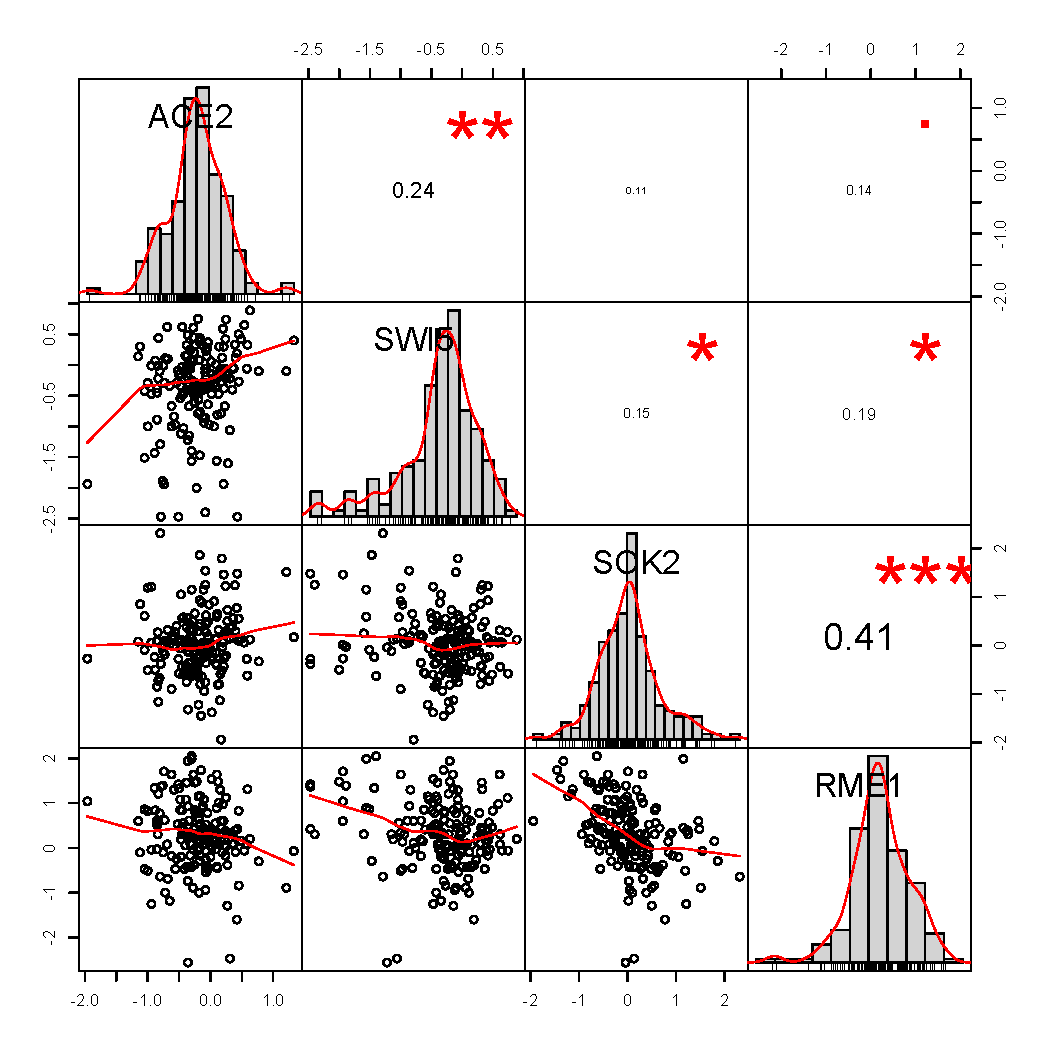
\includegraphics[width=0.5\columnwidth]{./figures/hands-on3/nice-pairs.pdf}
\caption{Output of the \lstinline!chart.Correlation()! function in the PerformanceAnalytics package, applied to the yeast expression data set.\label{fig:nicepairs}}
\end{figure}


% Here's an example based on code (see \href{http://gettinggeneticsdone.blogspot.com/2011/07/scatterplot-matrices-in-r.html}{this link} for the original source). Create a new R script called |mygraphs.R| and add the following function:
% %
% \begin{R}
% # panel.cor puts correlation in upper panels, size proportional to correlation
% panel.cor <- function(x, y, digits=2, prefix="", cex.cor, ...)
% {
%     usr <- par("usr"); on.exit(par(usr))
%     par(usr = c(0, 1, 0, 1))
%     r <- abs(cor(x, y))
%     txt <- format(c(r, 0.123456789), digits=digits)[1]
%     txt <- paste(prefix, txt, sep="")
%     if(missing(cex.cor))
%         cex.cor <- 0.8/strwidth(txt)
%     text(0.5, 0.5, txt, cex = cex.cor * r)
% }
% \end{R}
% You



\subsection{3D Scatter Plots}

A three-dimensional scatter plot can come in handy. The R library
\lstinline!lattice! has a function called \lstinline!cloud()! that
allows you to make such plots.
\begin{R}
> library(lattice)
> cloud(ACE2 ~ ASH1 * RAS2, data=yeast.clean)
> cloud(ACE2 ~ ASH1 * RAS2, data=yeast.clean, screen=list(x=-90, y=70)) # same plot from different angle
\end{R}
See the help file for \lstinline!cloud()! and \lstinline!panel.cloud()! for information on setting parameters.

\subsection{Scatterplot3D}
There is also a package available on CRAN called \lstinline!scatterplot3d! with similar functionality.
%
\begin{R}
> attach(yeast.clean) # so we can access the variables directly
> install.packages('scatterplot3d',dependencies=T) # installs scatterplot3d
> library(scatterplot3d) # assumes package is properly installed
> scatterplot3d(ASH1, RAS2, ACE2)
> scatterplot3d(ASH1, RAS2, ACE2, highlight.3d=T, pch=20,angle=25)
\end{R}
%
The |highlight.3d| argument colors points to help the viewer determine near and far points. Points that are closer to the viewer are lighter colors (more red in the default color scheme).

\subsubsection{Using Package Vignettes}
The Scatterplot3D package is quite flexible but this flexibility is hard to grok from the standard R help files (try |?scatterplot3d| to see for yourself).  Luckily the Scatterplot3D package includes a `vignette' -- a PDF document that discusses the design of the package and illustrates it's use.  Many packages include such vignettes. To see the list of vignettes available for your installed packages do the following:
%
\begin{R}
> vignette(all=T)
\end{R}
%
You should see that the vignette for the Scatterplot3D package is called |s3d|. You can access this vignette as follows, which should open the document in your default PDF viewer.
\begin{R}
> vignette("s3d")
\end{R}
%
In this case, the `good stuff' (i.e. the examples) starts on page 9 of the vignette.

\subsection{The rgl Package}

The 3D plots in |lattice| and |scatterplot3d| are fairly nice, but they don't allow the user to interact with the figures.  For example, wouldn't it be nice to be able to rotate a 3D scatter of points around to understand the relationships?  The |rgl| package allows you to do this, and can produce figures like that shown in Fig.~\ref{fig:rgl3d}.  Most R figures can be saved  using the |Save| option under the file menu. That's not the case for |rgl| plots. Instead we need to use the |rgl.postscript()| (creates a postscript or PDF version of the figure) or |snapshot3d()| (creates a screenshot) functions.
\begin{R}
> install.packages('rgl',dependencies=T)
> library(rgl)
> plot3d(ASH1, RAS2, ACE2, col='red', size=1, type='s')
> rgl.postscript('rgl3d-example.pdf', fmt='pdf')
\end{R}
%
\begin{figure}[htbp]
\centering
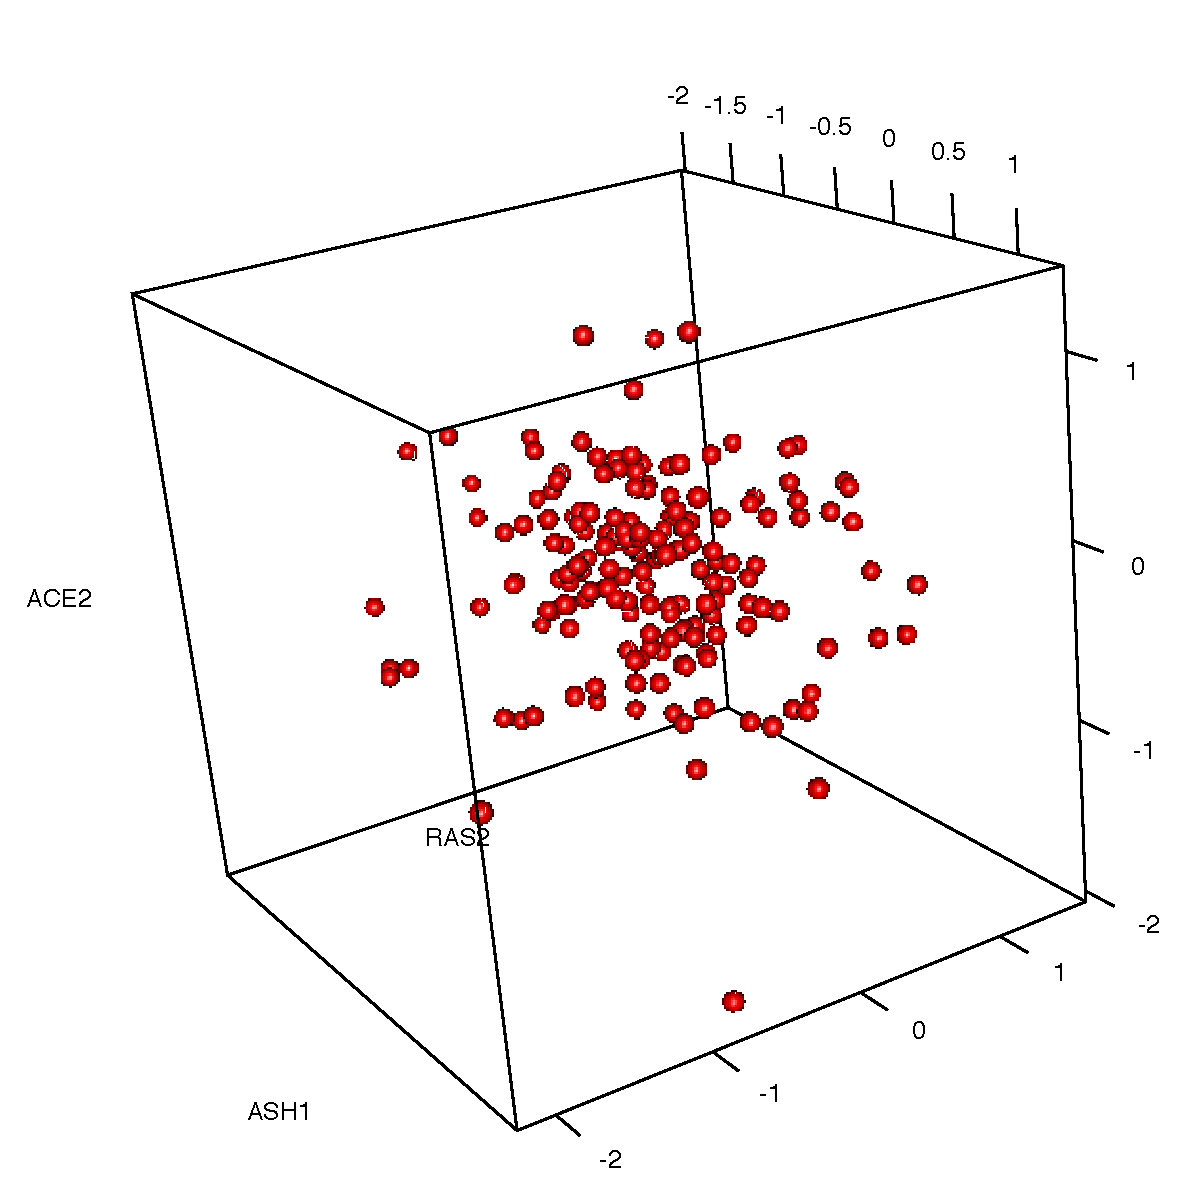
\includegraphics[width=0.5\columnwidth]{./figures/hands-on3/rgl3d-example.pdf}
\caption{Output of the \lstinline!plot3d()! function in the rgl package.\label{fig:rgl3d}}
\end{figure}

% Let's modify the 3D barplot on page 11 to create a 2D histogram. First we'll install another package -- |mvtnorm| -- that includes functions for creating multivariate normal distributions.
% %
% \begin{R}
% > install.packages('mvtnorm',dependencies=T)
% > library(mvtnorm)
% > ?rmvnorm # as always, check out the docs!

% \end{R}

\subsection{Colored grid plots}

A colored grid (or `heatmap') is another way of representing 3D data. It
most often is used to represent a variable of interest as a function of
two parameters. Grid plots can created using the \lstinline!image()!
function in R.

\begin{R}
> x <- seq(0, 2*pi, pi/20)
> y <- seq(0, 2*pi, pi/20)
> coolfxn <- function(x,y){
+    cos(x) * cos(y)}
> z <- outer(x,y,coolfxn) # the outer product of two matrices or vectors, see docs
> dim(z)
[1] 41 41
> image(x,y,z)
\end{R}
The \lstinline!x! and \lstinline!y! arguments to \lstinline!image()! are
vectors, the \lstinline!z! argument is a matrix (in this case created
using the outer product operator in conjunction with our function of
interest).

A somewhat more flexible function called |levelplot()| is found in the |lattice| package. For example, we can create a similar heatmap using |levelplot()| as follows:
\begin{R}
> library(lattice)
> levelplot(z)  # just the colors
> levelplot(z, contour=T) # colors plus contour lines
\end{R}
We can also apply the levelplot function to creat a representation of a correlation matrix, as shown here:
\begin{R}
> levelplot(cor(yeast.clean))
\end{R}
The default |levelplot()| colors are decent, but let's see how we can change the colors used to our liking. The |colorRampPalette()| function returns a function that interpolates between the values given as arguments to |colorRampPalette()|. So in the example below, it will create a series of colors from blue to white to red.
\begin{R}
> lvls <- seq(-1,1,0.1)  # set thresholds for our colors
> colors <- colorRampPalette(c('blue', 'white', 'red'))(length(lvls))
> levelplot(cor(yeast.clean), col.regions=colors, at=lvls)
\end{R}
%
The |colorRampPallete()| function can also take hexadecimal colors, as is commonly used in HTML. For a list of R colors see \url{http://research.stowers-institute.org/efg/R/Color/Chart/}.  For a  list of color schemes, developed by a geographer for effective cartographic representations,  see the \href{http://colorbrewer2.org/}{ColorBrewer web page}. For example, here's how to create the representation of the yeast data set correlation matrix shown in Fig.~\ref{fig:corrheat}:
\begin{R}
# this generates a color ramp from green to black to purple
> colors <- colorRampPalette(c('#1B7837', 'black', '#762A83'))(length(lvls))
> levelplot(cor(yeast.clean), col.regions=colors, at=lvls, scales=list(cex=0.6), xlab="", ylab="",main="Correlation Matrix\nYeast Expression Data")
\end{R}
The |scales| argument to |levelplot| changes the scaling of the tick marks and labels on the axes.

\begin{figure}[htbp]
\centering
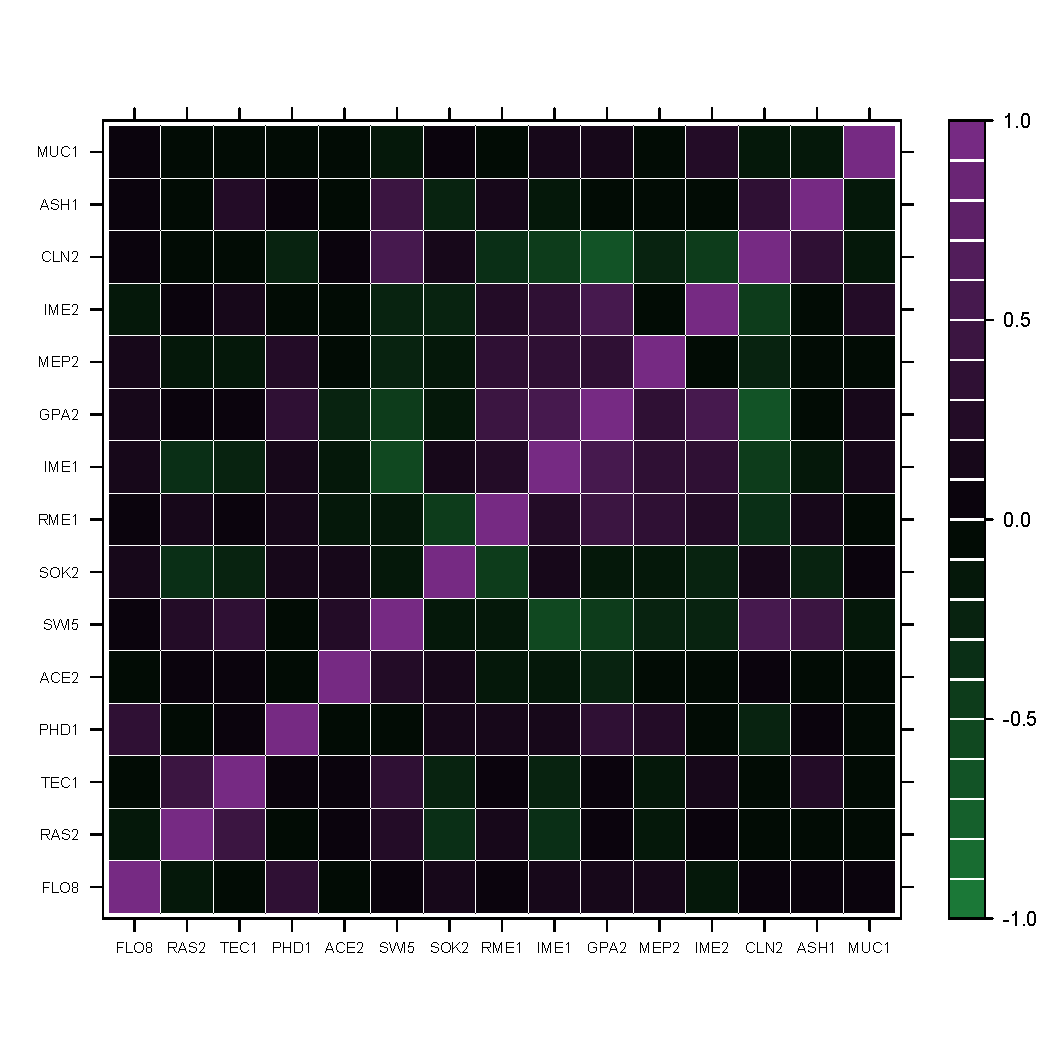
\includegraphics[width=0.5\columnwidth]{./figures/hands-on3/corr-heatmap.pdf}
\caption{A heatmap, representing the correlation matrix for the yeast expression data set, generated by the \lstinline!levelplot()! function in the lattice package.\label{fig:corrheat}}
\end{figure}

